\documentclass[11pt,a4paper]{article}
\usepackage[utf8]{inputenc}
\usepackage[vietnamese]{babel}
\usepackage{amsmath,amssymb}
\usepackage[version=4]{mhchem}
\usepackage{geometry}
\geometry{top=1.5cm,bottom=1.2cm,left=1.4cm,right=1.4cm,headheight=28pt,headsep=12pt,footskip=18pt}
\usepackage{graphicx}
\usepackage{xcolor}
\usepackage{tabularx}
\usepackage{array}
\usepackage{tikz}
\usepackage{fancyhdr}
\usepackage{enumitem}
\usepackage{multido}
\usepackage{tcolorbox}
\usepackage{colortbl}

\definecolor{hfRed}{HTML}{D32F2F}
\definecolor{hfGreen}{HTML}{8BC390}
\definecolor{mainGreen}{HTML}{2E7D32}
\definecolor{solBlue}{HTML}{1565C0}
\definecolor{tableGreen}{HTML}{E8F5E9}

\usepackage{ex_test}

\pagestyle{fancy}
\fancyhf{}
\renewcommand{\headrulewidth}{0.75pt}
\renewcommand{\headrule}{\hbox to\headwidth{\color{hfGreen}\leaders\hrule height \headrulewidth\hfill}}
\renewcommand{\footrulewidth}{0.75pt}
\renewcommand{\footrule}{\hbox to\headwidth{\color{hfGreen}\leaders\hrule height \footrulewidth\hfill}}

\fancyhead[L]{\small\itshape\color{hfRed}Tài liệu lưu hành nội bộ}
\fancyhead[R]{\small\color{hfRed}Thầy \textbf{TRẦN VĂN THẠNH} - 0777.470.803}

\fancyfoot[L]{\footnotesize\itshape\color{hfRed}CS1: 6/15 Nguyễn Hoàng, P. Kim Long, TP Huế \quad|\quad CS2: 24 Đặng Thái Thân, TP Huế}
\fancyfoot[R]{\small\textbf{\color{hfRed}Trang \thepage}}

\setlength{\parindent}{0pt}
\setlength{\parskip}{2pt}

\begin{document}

\begin{minipage}[t]{0.48\textwidth}
\textbf{SỞ GD\&ĐT THÀNH PHỐ HUẾ}\\
\textbf{TRƯỜNG THPT NGUYỄN CHÍ THANH}\\
\textit{ĐỀ CHÍNH THỨC}\\
\textit{(Đề có 04 trang)}
\end{minipage}
\hfill
\begin{minipage}[t]{0.48\textwidth}
\raggedleft
\textbf{\color{hfRed}ĐỀ KIỂM TRA GIỮA HỌC KỲ I – NĂM HỌC 2026 – 2027}\\
\textbf{MÔN HOÁ HỌC - LỚP 10}\\
\textit{Thời gian làm bài: 45 phút (không kể thời gian phát đề)}\\
\textbf{Mã đề: 1104}
\end{minipage}

\vspace{4pt}
\noindent
\textit{Họ tên:} \dotfill \textit{Lớp:} \dotfill \textit{Số báo danh:} \dotfill

\vspace{2pt}
\noindent
\textit{\footnotesize Cho biết nguyên tử khối (amu): $\ce{H = 1; C = 12; N = 14; O = 16; Na = 23; Mg = 24; Al = 27; P = 31; S = 32; Cl = 35{,}5; K = 39; Ca = 40; Fe = 56; Cu = 64; Zn = 65; Br = 80}$.\\
Cho biết số hiệu nguyên tử: $\ce{H = 1; Li = 3; C = 6; N = 7; O = 8; F = 9; Ne = 10; Na = 11; Mg = 12; Al = 13; Si = 14; P = 15; S = 16; Cl = 17; Ar = 18; K = 19; Ca = 20; Fe = 26; Cu = 29}$.}

\vspace{2pt}
\hrule color{hfGreen} height 0.5pt

\vspace{4pt}
\noindent
\textbf{\large\color{mainGreen}PHẦN I. Câu trắc nghiệm nhiều phương án lựa chọn: (16 câu – 4 điểm)}

\textit{Thí sinh trả lời từ câu 1 đến câu 16. Mỗi câu thí sinh chỉ chọn một phương án.}
\vspace{4pt}

\begin{ex}%[1104-C1]
Các đồng vị của cùng một nguyên tố hóa học là những nguyên tử có
\choice
{cùng số neutron nhưng khác nhau về số proton.}
{cùng số khối $A$ nhưng khác nhau về số proton.}
{cùng tổng số hạt proton và neutron nhưng khác nhau về số electron.}
{\True cùng số proton nhưng khác nhau về số neutron.}

\end{ex}

\begin{ex}%[1104-C2]
Cấu hình electron nguyên tử của potassium ($Z = 19$) là $1s^2 2s^2 2p^6 3s^2 3p^6 4s^1$. Vị trí của potassium trong bảng tuần hoàn là
\choice
{ô số 19, chu kì 4, nhóm IB.}
{ô số 19, chu kì 3, nhóm IA.}
{\True ô số 19, chu kì 4, nhóm IA.}
{ô số 19, chu kì 1, nhóm IVA.}

\end{ex}

\begin{ex}%[1104-C3]
Nguyên tử của nguyên tố phosphorus có $Z = 15$ và $A = 31$. Số hạt neutron trong nguyên tử phosphorus là
\choice
{\True 16.}
{31.}
{46.}
{15.}

\end{ex}

\begin{ex}%[1104-C4]
Cho các nguyên tử sau: $^{12}_{6}\text{X}$, $^{14}_{7}\text{Y}$, $^{13}_{6}\text{Z}$, $^{16}_{8}\text{T}$. Hai nguyên tử nào là đồng vị của cùng một nguyên tố hóa học?
\choice
{$\text{X}$ và $\text{Y}$.}
{\True $\text{X}$ và $\text{Z}$.}
{$\text{Z}$ và $\text{T}$.}
{$\text{Y}$ và $\text{T}$.}

\end{ex}

\begin{ex}%[1104-C5]
Số orbital trong các phân lớp s, p, d lần lượt bằng
\choice
{\True 1, 3, 5.}
{1, 2, 3.}
{1, 2, 4.}
{3, 5, 7.}

\end{ex}

\begin{ex}%[1104-C6]
Số electron tối đa có thể chứa trong lớp thứ $n$ (với $n \le 4$) được tính theo công thức là
\choice
{$2n + 1$.}
{\True $2n^2$.}
{$2n$.}
{$n^2$.}

\end{ex}

\begin{ex}%[1104-C7]
Kí hiệu chung của nguyên tử là $^{A}_{Z}\text{X}$, trong đó $A$ và $Z$ lần lượt biểu diễn cho
\choice
{số hiệu nguyên tử và số khối.}
{số khối và số neutron.}
{\True số khối và số hiệu nguyên tử.}
{số neutron và số hiệu nguyên tử.}

\end{ex}

\begin{ex}%[1104-C8]
Bảng tuần hoàn các nguyên tố hoá học được sắp xếp không tuân theo nguyên tắc nào sau đây?
\choice
{Các nguyên tố mà nguyên tử có cùng số lớp electron được xếp vào một hàng.}
{Các nguyên tố mà nguyên tử có cùng số electron hoá trị được xếp vào một cột.}
{Các nguyên tố được sắp xếp theo chiều tăng dần của điện tích hạt nhân nguyên tử.}
{\True Các nguyên tố được sắp xếp theo chiều tăng dần khối lượng nguyên tử.}

\end{ex}

\begin{ex}%[1104-C9]
Orbital nguyên tử (AO) là
\choice
{quỹ đạo chuyển động có hình tròn xác định của electron xung quanh hạt nhân.}
{\True khu vực không gian xung quanh hạt nhân mà tại đó xác suất tìm thấy electron là lớn nhất.}
{đám mây hình bầu dục chứa tất cả các electron của nguyên tử.}
{đường tròn trên đó các electron chuyển động với tốc độ không đổi.}

\end{ex}

\begin{ex}%[1104-C10]
Nguyên tố hóa học là tập hợp các nguyên tử có cùng
\choice
{số khối $A$.}
{tổng số proton và neutron.}
{\True số proton.}
{số neutron.}

\end{ex}

\begin{ex}%[1104-C11]
Đồng có hai đồng vị bền trong tự nhiên là $^{63}_{29}\ce{Cu}$ và $^{65}_{29}\ce{Cu}$. Nguyên tử khối trung bình của đồng là 63,55 (điện tích $z$ của các ion đồng vị bền đều bằng $+1$). Hình vẽ phổ khối nào dưới đây là đúng?
\begin{center}
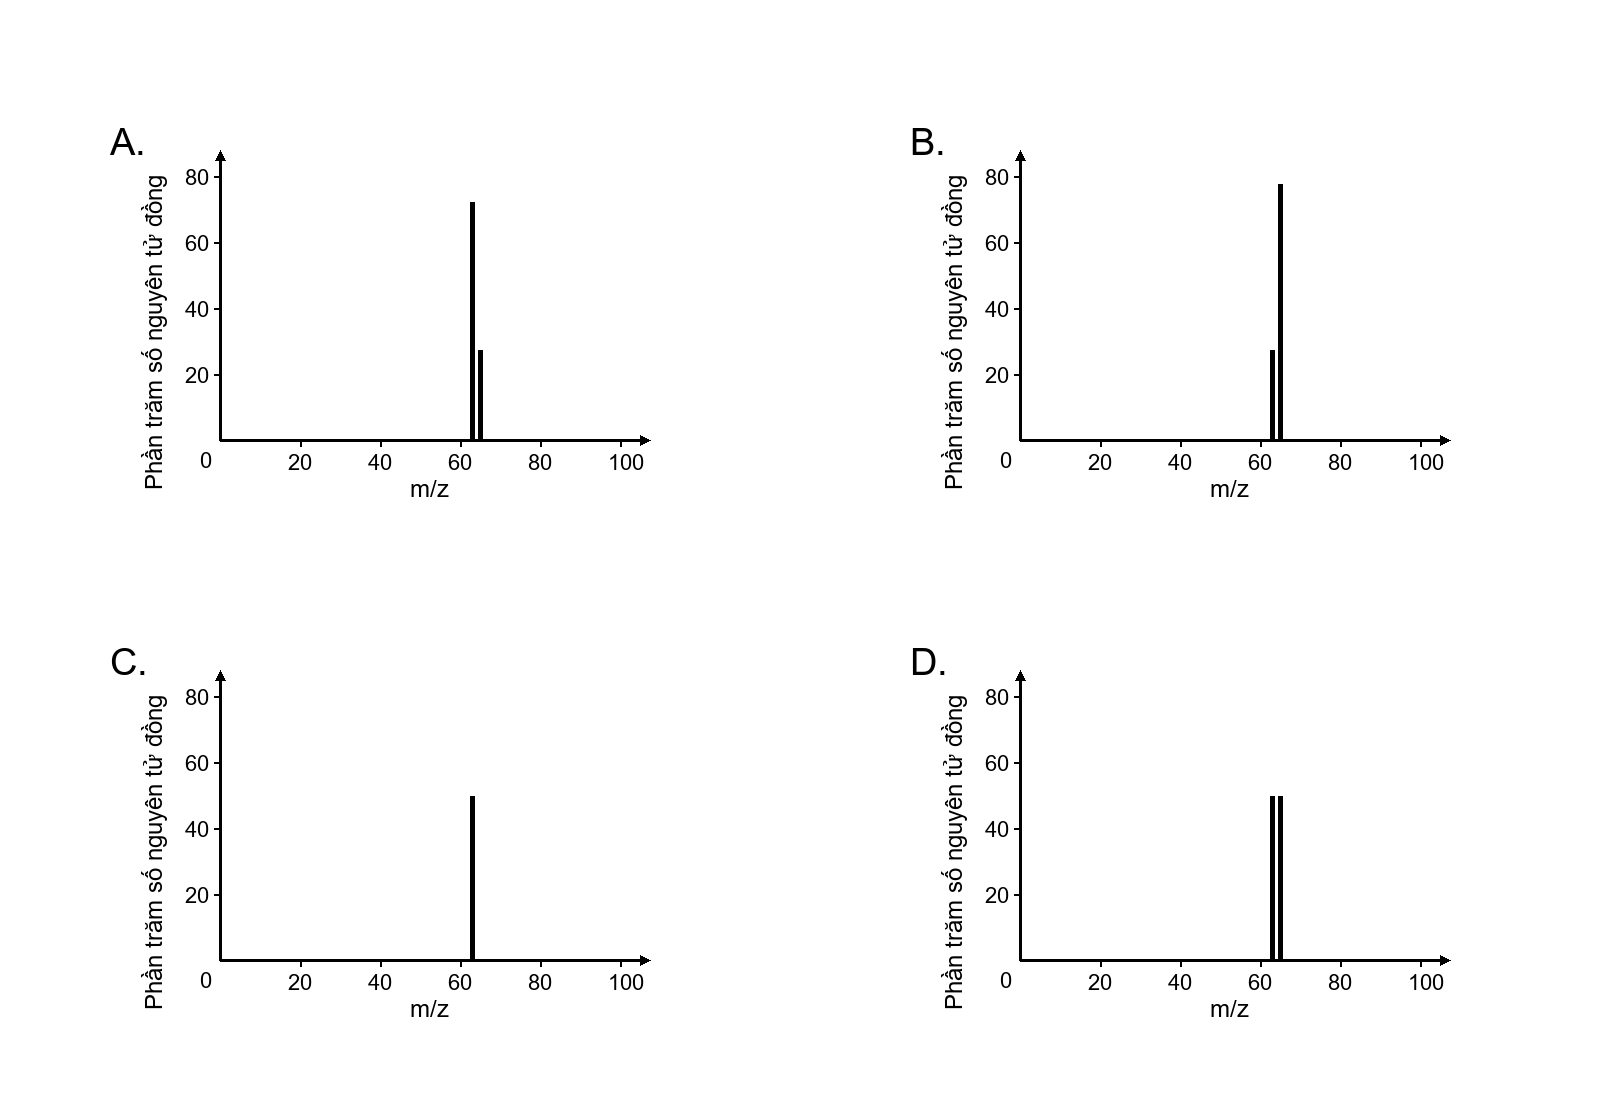
\includegraphics[width=13.5cm]{images_hoa10/pho_khoi_cu_ma1104.png}
\end{center}
\choice
{\True Hình A.}
{Hình B.}
{Hình C.}
{Hình D.}

\end{ex}

\begin{ex}%[1104-C12]
Trong nguyên tử, loại hạt nào có khối lượng không đáng kể so với các hạt còn lại?
\choice
{Neutron.}
{Proton.}
{Neutron và electron.}
{\True Electron.}

\end{ex}

\begin{ex}%[1104-C13]
Bảng tuần hoàn hiện nay gồm có bao nhiêu chu kì?
\choice
{\True 7.}
{18.}
{8.}
{6.}

\end{ex}

\begin{ex}%[1104-C14]
Khối lượng của nguyên tử magnesium là $39{,}8271\cdot 10^{-27}\,\text{kg}$. Khối lượng của magnesium theo amu là
\choice
{24,000.}
{$23{,}985\cdot 10^{-3}$.}
{\True 23,978.}
{$66{,}133\cdot 10^{-51}$.}

\end{ex}

\begin{ex}%[1104-C15]
Hạt nhân của hầu hết các nguyên tử đều được tạo nên từ các loại hạt là
\choice
{\True proton và neutron.}
{neutron và electron.}
{electron, proton và neutron.}
{electron và proton.}

\end{ex}

\begin{ex}%[1104-C16]
Cấu hình electron của nguyên tử $\ce{Ca}$ ($Z = 20$) ở trạng thái cơ bản là
\choice
{$1s^2 2s^2 2p^6 3s^2 3p^6 4p^2$.}
{$1s^2 2s^2 2p^6 3s^2 3p^6 4s^2 4p^1$.}
{\True $1s^2 2s^2 2p^6 3s^2 3p^6 4s^2$.}
{$1s^2 2s^2 2p^6 3s^2 3p^6 4s^1$.}

\end{ex}

\vspace{6pt}
\noindent
\textbf{\large\color{mainGreen}PHẦN II. Câu trắc nghiệm đúng sai: (2 câu – 2 điểm)}

\textit{Thí sinh trả lời từ câu 1 đến câu 2. Trong mỗi ý a), b), c), d) ở mỗi câu thí sinh chọn đúng hoặc sai.}
\vspace{4pt}

\begin{ex}%[1104-P2-C1]
Cho nguyên tử iron ($\ce{Fe}$) có kí hiệu nguyên tử là $^{56}_{26}\ce{Fe}$. Biết nguyên tử $\ce{Fe}$ có cấu hình electron viết gọn là $[\ce{Ar}]3d^6 4s^2$.
\choiceTF
{\True Nguyên tử $\ce{Fe}$ có 26 hạt proton, 26 hạt electron và 30 hạt neutron}
{\True Nguyên tố $\ce{Fe}$ thuộc chu kì 4, nhóm VIIIB trong bảng tuần hoàn}
{Lớp vỏ nguyên tử $\ce{Fe}$ có 8 electron ở lớp ngoài cùng}
{Cation $\ce{Fe^{2+}}$ được tạo thành khi nguyên tử $\ce{Fe}$ nhường đi 2 electron ở phân lớp 3d}

\end{ex}

\begin{ex}%[1104-P2-C2]
Nguyên tố X được dùng để chế tạo hợp kim nhẹ, bền, dùng trong nhiều lĩnh vực: hàng không, ô tô, xây dựng, hàng tiêu dùng... Nguyên tố Y ở dạng $\ce{YO4^{3-}}$, đóng vai trò quan trọng trong các phân tử sinh học như DNA và RNA. Các tế bào sống sử dụng $\ce{YO4^{3-}}$ để vận chuyển năng lượng. Nguyên tử của nguyên tố X có cấu hình electron kết thúc ở phân lớp $3p^1$. Nguyên tử của nguyên tố Y có cấu hình electron kết thúc ở phân lớp $3p^3$.
\choiceTF
{\True Cấu hình electron của X là $[\ce{Ne}]3s^2 3p^1$}
{\True Cấu hình electron của Y là $[\ce{Ne}]3s^2 3p^3$}
{\True Y là phi kim}
{\True X là kim loại}

\end{ex}

\vspace{6pt}
\noindent
\textbf{\large\color{mainGreen}PHẦN III. Câu trắc nghiệm trả lời ngắn: (4 câu – 1 điểm)}

\textit{Thí sinh trả lời từ câu 1 đến câu 4.}
\vspace{4pt}

\begin{ex}%[1104-P3-C1]
Aluminium là kim loại phổ biến nhất trên vỏ Trái Đất, được sử dụng trong các ngành xây dựng, ngành điện hoặc sản xuất đồ gia dụng. Hạt nhân của nguyên tử aluminium có điện tích bằng $+13$ và số khối bằng 27. Số neutron có trong nguyên tử aluminium là bao nhiêu?

\textbf{Trả lời: } \dotfill

\end{ex}

\begin{ex}%[1104-P3-C2]
Cho các nguyên tố hóa học có số hiệu nguyên tử lần lượt là: $Z_1 = 7; Z_2 = 11; Z_3 = 12; Z_4 = 16; Z_5 = 17; Z_6 = 18$. Trong số các nguyên tố trên, có bao nhiêu nguyên tố là phi kim?

\textbf{Trả lời: } \dotfill

\end{ex}

\begin{ex}%[1104-P3-C3]
Nguyên tử của nguyên tố calcium ($Z = 20$) ở trạng thái cơ bản có bao nhiêu orbital nguyên tử chứa electron?

\textbf{Trả lời: } \dotfill

\end{ex}

\begin{ex}%[1104-P3-C4]
Nguyên tố X được sử dụng rộng rãi trong đời sống: đúc tiền, làm đồ trang sức, làm răng giả,... Muối iodide của X được sử dụng nhằm tụ mây tạo ra mưa nhân tạo. Tổng số hạt cơ bản trong nguyên tử nguyên tố X là 155, số hạt mang điện nhiều hơn số hạt không mang điện là 33 hạt. Số khối của nguyên tử X là bao nhiêu?

\textbf{Trả lời: } \dotfill

\end{ex}

\vspace{6pt}
\noindent
\textbf{\large\color{mainGreen}PHẦN IV. TỰ LUẬN: (3 câu – 3 điểm)}

\textit{Thí sinh trả lời từ câu 1 đến câu 3.}
\vspace{4pt}

\begin{ex}%[1104-TL1]
\textbf{(1,0 điểm)} Nguyên tố boron (B) có nguyên tử khối trung bình là 10,81. Trong tự nhiên, boron có hai đồng vị bền là $^{10}\text{B}$ và $^{11}\text{B}$.
\begin{enumerate}[label=\textbf{\alph*)}]
\item Tính phần trăm số nguyên tử của mỗi đồng vị trong tự nhiên.
\item Tính phần trăm khối lượng của đồng vị $^{11}\text{B}$ có trong hợp chất boric acid $\ce{H3BO3}$ (cho biết nguyên tử khối của $\ce{H = 1; O = 16}$).
\end{enumerate}

\noindent\textit{Bài làm:}
\multido{\i=1+1}{8}{\noindent\makebox[\linewidth]{\dotfill}\\[1.5pt]}

\end{ex}

\begin{ex}%[1104-TL2]
\textbf{(1,0 điểm)} Nguyên tử của nguyên tố X có tổng số electron trên các phân lớp p là 8.
\begin{enumerate}[label=\textbf{\alph*)}]
\item Viết cấu hình electron đầy đủ và cấu hình electron theo ô orbital của nguyên tử X.
\item Xác định vị trí của X trong bảng tuần hoàn (ô số, chu kì, nhóm). Giải thích ngắn gọn.
\end{enumerate}

\noindent\textit{Bài làm:}
\multido{\i=1+1}{8}{\noindent\makebox[\linewidth]{\dotfill}\\[1.5pt]}

\end{ex}

\begin{ex}%[1104-TL3]
\textbf{(1,0 điểm)} Hợp chất có công thức $\ce{M2X}$ (được sử dụng trong sản xuất xi măng, phân bón) có tổng số hạt là 140. Trong đó số hạt mang điện nhiều hơn số hạt không mang điện là 44. Số khối của M lớn hơn số khối của X là 23. Tổng số hạt trong nguyên tử M nhiều hơn trong nguyên tử X là 34. Xác định công thức phân tử của hợp chất $\ce{M2X}$, gọi tên tiếng anh và phân loại các nguyên tố M và X theo cấu hình electron (nguyên tố s, p, d, f).

\noindent\textit{Bài làm:}
\multido{\i=1+1}{12}{\noindent\makebox[\linewidth]{\dotfill}\\[1.5pt]}

\end{ex}

\vspace{8pt}
\begin{center}
\textbf{---------------------- HẾT ----------------------}
\end{center}
\begin{center}
\textit{\small - Thí sinh không được sử dụng tài liệu.\\ - Cán bộ coi thi không giải thích gì thêm.}
\end{center}

\end{document}
